\begin{comment}
\chapter{Koncepcja rozwiązania}
\label{chapter:koncepcjarozwiazania}

W niniejszym rozdziale skupiam się na opisie koncepcji rozwiązania wykorzystania
analizy sentymentu, sieci społecznych i geolokacji w analizie zachowań
użytkowników serwisów społecznościowych. W kolejnych podrozdziałach opisuję
sposoby w jaki dane zagadnienia zostały zaaplikowane w moich badaniach.
Na początku przedstawiam gruboziarnisty model systemu (\ref{section:modelsystemu}),
który prezentuje jego najważniejsze moduły. Następnie opisuję tematykę
i sposób gromadzenia danych (\ref{section:gromadzeniedanych}) potrzebnych do 
przeprowadzenia analizy internautów. Później omawiam metodę jaką zastosowałem 
podczas analizy sentymentu (\ref{section:analizasentymentu}) wpisów użytkowników.
W dalszej kolejności skupiam się nad zastosowanymi
sposobami analizy sieci społecznych (\ref{section:siecispoleczne})
i całość kończę omówieniem wykorzystania geolokacji w moich badaniach 
(\ref{section:wykorzystaniegeolokacji}).








%%%%%%%%%%%%%%%%%%%%%%%%%%%%%%%%%%%%%%%%%%%%%%%%%%%%%%%%%%%%%%%% MODEL SYSTEMU
\section{Model systemu}
\label{section:modelsystemu}
Stworzony system zbudowany jest z kilku modułów. Wyróżnić można jego
trzy główne części:
\begin{itemize}
  \item gromadzenie danych,
  \item przetwarzanie danych,
  \item analiza zebranych danych.
\end{itemize} 
Wszystkie informacje zapisywanie są w jednej, centralnej bazie danych.
Schemat systemu zaprezentowany jest na rysunku 
\ref{image:gruboziarnisty-model-systemu}.


\clearpage

\begin{figure}[ht!]
\centering
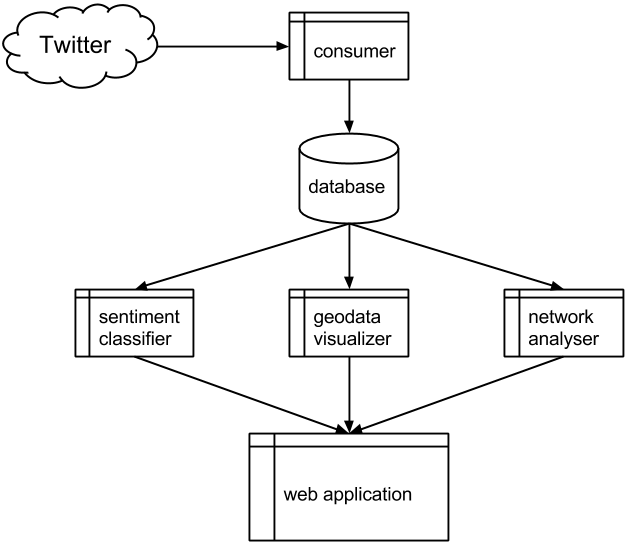
\includegraphics[width=140mm]{img/budowa-systemu.png}
\caption{Gruboziarnisty model systemu}
\label{image:gruboziarnisty-model-systemu}
\end{figure}

Każda z wyróżnionych powyżej części systemu bierze udział w innym etapie
badań. Na początku najważniejsze jest gromadzenie danych, po którym następuje
ich przetwarzanie by na końcu zająć się analizą i próba ekstrakcji wiedzy.
Wszystkie te części są ze sobą połączone wspólną bazą danych, w której
przechowywana jest zgromadzona wiedza i wyniki przetwarzania i analizy danych.
Poniżej pokrótce omówione są wszystkie z tych części.  

%%%%%%%%%%%%%%%%%%%%%%%%%%%%%%%%%%%%%%%%%%%%%%%%%%%%%%%%%%%% GROMADZENIE DANYCH
\section{Gromadzenie danych}
\label{section:gromadzeniedanych}
W tej sekcji opisuję sposób przeprowadzenia początkowych prac związanych
z moimi badaniami, które związane były ze zgromadzeniem danych potrzebnych
do przeprowadzania analiz. Etap ten był niezwykle istotny i przeprowadzenie
go umożliwiło dalsze prace. Zgromadzone dane pochodzą z serwisu Twitter
i zostały uzyskane przy pomocy udostępnionego publicznie 
API (interfejsu
programistycznego).

\subsection{Tematyka danych}
% piłka nożna, kibice
Aby przeprowadzić analizę danych koniecznym było wybranie podzbioru
użytkowników Twittera. Dwa aspekty zadecydowały o tym, że skupiono się nad
analizą anglojęzycznego środowiska piłkarskiego:
\begin{itemize}   
  \item struktura językowa użytkowników sieci Twitter -- według badań firmy Gnip
  \cite{GnipTwitterLanguages} (zajmującej się gromadzeniem danych z tego serwisu
  społecznościowego) w 2013 roku ponad 50\% tweetów wysłanych zostało w języku
  angielskim.
  Dla porównania w języku polskim było to zaledwie 0.11\%.
  Dlatego też badanie użytkowników anglojęzycznych ma największy sens, gdyż
  prowadzi do zebrania największej liczby tweetów.
  Wybór konkretnego języka komunikacji jest o tyle istotny, iż wpływa znacznie
  na część badań związaną z analizą sentymentu,
  \item dynamika wpisów na Twitterze -- w związku z narzuconym w serwisie
  ograniczeniem na liczbę znaków wpisu (140) oraz sposobem ich prezentowania
  użytkownikom na ich stronie głównej (chronologicznie od najnowszych) serwis
  ten charakteryzuje się wysoką dynamiką informacji wysyłanych przez użytkowników.
  Wpisy bardzo często odnoszą się do aktualnych wydarzeń, krótko je komentując.
  W związku z tym badanie środowiska piłkarskiego ma duży sens, gdyż zainteresowani
  futbolem internauci mają wiele tematów do dyskusji -- komentowanie spotkań na żywo,
  refleksje po meczach i dyskusje między spotkaniami.
  W profesjonalnych ligach piłkarskich mecze odbywają się co najmniej raz w tygodniu,
  a informacje o stanie kadrowym, kontuzjach i nadziejach przed meczem
  rozpalają kibiców swoich drużyn. W związku z wysoką dynamiką świata piłkarskiego,
  użytkownicy Twittera będący kibicami tworzą proporcjonalnie dużą liczbę
  tweetów -- komentując na biężąco wszelkie wydarzenia. Dlatego też wybór
  tej podgrupy do moich badań jest racjonalny i daje możliwość zbadania 
  zachowań użytkowników społecznościowych dostarczając wiele wpisów, na których
  można przeprowadzić analizy.
\end{itemize}  


\subsection{Sposób zbierania danych}
% wybrane kluby, słowa kluczowe, API, nasłuchiwanie
Aby uzyskać jak najlepsze rezultaty zbierania danych ze środowiska piłkarskiego
(posługującego się językiem angielskim) jako dziedzinę badań wybrano
najwyższą klasę rozgrywek piłki nożnej mężczyzn w Anglii (i Walii),
czyli Premier Leauge -- uznawaną przez wielu ekspertów za najsilniejszą ligę na
świecie. Co istotne, jest to także najczęściej oglądana liga piłkarska.
Średnio pojedynczy mecz ma widownię ponad 12 milionów osób
\cite{PremierLeagueAudience} bijąc ponad dwukrotnie oglądalność innych lig 
(włoskiej, hiszpańskiej czy niemieckiej).

Zbieranie danych odbywało się przy pomocy Twitter Stream API. Do nasłuchiwania
wpisów koniecznym jest także zdefiniowanie filtrów określających jakie dane nas
interesują. Zdecydowałem się korzystać z filtra słów kluczowych wraz z
ograniczeniem wpisów na język angielski.

Twitter Stream API dostarcza jedynie tweety pojawiających się w czasie
rzeczywistym. Oznacza to, że możemy przy jego użyciu mieć jedynie dostęp do tych
wpisów, które zostały wysłane, gdy jednocześnie uruchomiony był nasz program
nasłuchujący. Aby zmaksymalizować jakość i zakres zebranych danych program
nasłuchujący uruchamiany był w trakcie odbywania się meczów 
(z kilkudziesięciuminutowym zapasem czasowym przed i po spotkaniu).

W związku z koniecznością określania słów kluczowych ograniczono liczbę
śledzonych klubów do najlepszej czwórki sezonu 2012/2013, którą tworzą:
Manchester United FC, Manchester City FC, Chelsea FC oraz Arsenal FC.
Są to więc odpowiednio dwa kluby z Manchesteru i dwa z Londynu.

Mecze nasłuchiwano od 23 listopada do 29 grudnia 2013 roku. W tym czasie odbyło
się 9 kolejek spotkań (od 12 do 19 kolejki włącznie). Jako słowa kluczowe przed
każdym meczem definiowane były: nazwiska i znane określenia
piłkarzy, nazwiska i znane określenia trenerów (menadżerów) drużyn, nazwy i
określenia klubów, nazwisko głównego sędziego i nazwa stadionu. 
Oprócz meczów Premier League nasłuchiwano także dwóch kolejek Ligi Mistrzów
z udziałem wyżej wymienionych zespołów, które odbyły się w tym czasie.


%%%%%%%%%%%%%%%%%%%%%%%%%%%%%%%%%%%%%%%%%%%%%%%%%%%%%%%%%%%% ANALIZA SENTYMENTU
\section{Analiza sentymentu}
\label{section:analizasentymentu}
W tym miejscu opisuję sposób w jaki została użyta do moich badań analiza
wydźwięku wypowiedzi. Przedstawiam czynności wstępne jakie zostały zastosowane
na tekście, prezentuję krótko wybrany algorytm i zastosowane w nim modyfikacje
oraz opisuję sposób zaaplikowania analizy wydźwięku na zgromadzonych tweetach.

\subsection{Normalizacja tekstu}
% pozbycie się słów kluczowych, zaprzeczenia, retweety

W związku z tym, że wpisy są tworzone przez zwykłych użytkowników posiadają one
wiele znaków i elementów, które z punktu widzenia analizy sentymentu są zbędne,
a czasami prowadzące do błędów. Dlatego też tekst należy poddać normalizacji,
usunięciu zbędnych elementów, szumów i spamu. Przykładowa lista wpisów jakie
znalazły się w zgromadzonych danych przedstawia poniższa tabela
(\ref{tab:wpisy-przed-normalizacja}).


\begin{table}[ht!]  
\begin{center}  
\begin{tabular}{|r|p{140mm}|}
\hline
\multicolumn{2}{|c|}{Przed normalizacją}
\\ \hline
1 & RT @J\_SPEKZ: Haha quality! \#Fellaini \#United \#Moyes
http://t.co/rJB4K1fvZy
\\ \hline
2 & Stay woke brah! The Arsenal is about to make everything alright soon :) RT
@JCphoenixx: So damn tired, So not sleepy.
\\ \hline
3 & @abdul1haseeb My arsenal is not disappointing too :P 
\\ \hline
4 & @Arsenal didn't think i could respect @aaronramsey any more than i already
did, bute what a gentleman he is for not to celebrate that goal:) 
\\ \hline
5 & OHHHHHH!!!!! SO CLOSE!!! Wilshere!!! Good Job Ramsey keeping that move alive
\\ \hline
6 & Haha, you gotta agree, no one gets booed like Manchester United :D \#ZeDevilza
\\
\hline
\end{tabular} 
\end{center} 
\caption{Przykładowa lista wpisów przed normalizacją}
\label{tab:wpisy-przed-normalizacja}
\end{table}


\clearpage
Po przeprowadzeniu wszystkich prac związanych z normalizacją tekstu wpisy z
powyższej tabeli prezentują się w następujący sposób:

\begin{table}[ht!]  
\begin{center}  
\begin{tabular}{|r|p{140mm}|}
\hline
\multicolumn{2}{|c|}{Po normalizacji}
\\ \hline
1 & 
\\ \hline
2 & stay woke brah make alright
\\ \hline
3 & not\_disappointing
\\ \hline
4 & didnt not\_respect bute gentleman not\_celebrate not\_goal
\\ \hline
5 & ohhhhhh close good job keeping alive
\\ \hline
6 & haha gotta agree not\_booed
\\
\hline
\end{tabular} 
\end{center} 
\caption{Lista wpisów poddanych normalizacji}
\label{tab:wpisy-po-normalizacja}
\end{table}

Kolejne kroki, które przekształciły tweety do powyższej postaci to:
\begin{enumerate}
  \item Usunięcie skomentowanych retweetów.\\
  \texttt{Stay woke brah! The Arsenal is about to make everything
  alright soon :) \sout{RT @JCphoenixx: So damn tired, So not sleepy.}}
  
  \item Usunięcie skomentowanych cytowań. \\
  \texttt{At all...\sout{"@dotun\_somoye: Even city's first goal
  negredo was offside....:( the refs not helping at all"} }
  
  \item Usunięcie hiperlinków.\\
  \texttt{You up for Arsenal's match later on? - what time? maybe if i'm not
  busy baby sitting :) \sout{http://t.co/aC5Ec8ipy1}}
 
  
  \item Usunięcie nazw użytkowników.\\
  \texttt{\sout{@abdul1haseeb} My arsenal is not disappointing too :P}
  
  
  \item Usunięcie hashtagów. \\
  \texttt{Haha, you gotta agree, no one gets booed like Manchester United :D
  \sout{\#ZeDevilza}}
  
  
  \item Oznaczenie wyrazów zaprzeczonych przedrostkiem \texttt{NOT\_} (opisuję
  dokładniej w sekcji \ref{subsection:sentyment-algorytm}). \\
  \texttt{didn't \textbf{NOT\_think NOT\_i NOT\_could NOT\_respect NOT\_any 
  NOT\_more NOT\_than NOT\_i NOT\_already NOT\_did}, bute what a gentleman he 
  is for not \textbf{NOT\_to NOT\_celebrate NOT\_that NOT\_goal:)}}

 \item Zachowanie tylko znaków alfabetu:
  	\begin{itemize}
  		\item usunięcie zaimków dzierżawczych (\texttt{Helen's} $\to$ \texttt{Helen}),
  		\item usunięcie apostrofu ze skróconych zaprzeczeń (\texttt{don't} $\to$ \texttt{dont}),
  		\item normalizacja liter diakrytyzowanych (\texttt{José Mourinho} $\to$ \texttt{Jose
  		Mourinho})
  		\item usunięcie liczb i wszelkich znaków niealfabetycznych.
	\end{itemize}

  \texttt{You up for Arsenal\sout{'s} match later on\sout{? -} what
  time\sout{?} maybe if i\sout{'}m not busy baby sitting \sout{:)}} 
	
	\item Usunięcie wyrazów zdefiniowanych w stop liście (powszechne wyrazy danego
	języka, które mogą być pominięte nie tracąc jednocześnie żadnej informacji).
	Zastosowałem stop listę z serwisu \mbox{WebPageAnalyse.com} 
	\cite{WebPageAnalyse} zawierającą 528 słów.

	\texttt{\sout{You up for} Arsenal match \sout{later on what} time \sout{maybe if} 
 	im \sout{not} busy baby sitting}
	
	\item Usunięcie słów kluczowych, które użyte były do gromadzenia wpisów z
	Twittera -- czyli nazwisk piłkarzy, menadżerów, nazw klubów, itd.
	
	%\texttt{\sout{BENDTNER} FUCKING im \sout{NOT\_arsenal} NOT\_fan}
	
	\texttt{OHHHHHH CLOSE \sout{Wilshere} Good Job \sout{Ramsey} keeping alive}
	
\end{enumerate}





\subsection{Zastosowanie algorytmu}
\label{subsection:sentyment-algorytm}
% + dobór parametrów, emotikony, zaprzeczenia

Do przeprowadzenia analizy sentymentu na zebranych tweetach skorzystałem z
metody opracowanej przez Alexandra Paka i Patricka Paroubek'a, którą krótko
przedstawiłem w sekcji \ref{subsubsection:pakandparoubek}.
Jest to technika, która pozwala badać sentyment nie posiadając wcześniej
słownika sentymentu. Dlatego też pierwszym krokiem jest zbudowanie takiego
słownika z zebranych danych.
W tym celu wybiera się podzbiór wpisów, które zawierają emotikony.
W związku ze 140 znakowym ograniczeniem na długość znaków przyjmuje się
założenie, że dana emotikona nadaje wydźwięk całemu wpisowi.
Według artykułu \cite{EmoticonAnalysisTwitter} 20 emotikon pokrywa w 90\%
stosowanie tych znaków graficznych we wpisach (na 100 wpisów z emotikonami, 90 z
nich zawiera emotikonę ze zbioru tych 20). Dlatego też skorzystałem z tego
zbioru do własnych badań dzieląc emotikony na wyrażające wydźwięk pozytywny i
negatywny w sposób\footnote{emotikona \texttt{D:} została pominięta, gdyż
pokrywała więcej przypadków niż tylko użycie emotikony (np.:
\texttt{Accepte\textbf{d:} Mary, John, Jane})} przedstawiony w tabeli
\ref{tab:wydzwiek-emotikon}.

\begin{table}[ht!]  
\begin{center}  
\begin{tabular}{|c|r|l|}
\hline
Emotikona & Popularnoś według \cite{EmoticonAnalysisTwitter} &
Wydźwięk \\ \hline
\texttt{:)} & $33.4\%$ & pozytywny \\ \hline
\texttt{:D} & $11.0\%$ & pozytywny \\ \hline
\texttt{:(} & $7.9\%$ & negatywny \\ \hline
\texttt{;)} & $7.5\%$ & pozytywny \\ \hline
\texttt{:-)} & $4.4\%$ & pozytywny \\ \hline
\texttt{:P} & $3.7\%$ & pozytywny \\ \hline
\texttt{=)} & $3.7\%$ & pozytywny \\ \hline
\texttt{(:} & $2.8\%$ & pozytywny \\ \hline
\texttt{;-)} & $2.2\%$ & pozytywny \\ \hline
\texttt{:/} & $1.9\%$ & negatywny \\ \hline
\texttt{XD} & $1.9\%$ & pozytywny \\ \hline
\texttt{=D} & $1.5\%$ & pozytywny \\ \hline
\texttt{:O} & $1.1\%$ & pozytywny \\ \hline
\texttt{=]} & $1.1\%$ & pozytywny \\ \hline
\texttt{;D} & $1.0\%$ & pozytywny \\ \hline
\texttt{:]} & $1.0\%$ & pozytywny \\ \hline
\texttt{:-(} & $0.8\%$ & negatywny \\ \hline
\texttt{=/} & $0.8\%$ & negatywny \\ \hline
\texttt{=(} & $0.8\%$ & negatywny \\ \hline
\end{tabular} 
\end{center} 
\caption{Wydźwięk emotikon}
\label{tab:wydzwiek-emotikon}
\end{table}

Następnie przeglądnięto wszystkie tweety z emotikonami zliczając liczbę
występowania wyrazów w kontekście pozytywnym i negatywnym.
Najpierw badano sentyment całego wpisu (na podstawie emotikony -- gdy była ich
większa ilość wybierano ten sentyment, który przeważał) a następnie dla każdego
wyrazu z tego wpisu zwiększano licznik odpowiednio wystąpień pozytywnych lub
negatywnych. Oczywiście wpisy były już poddane normalizacji.
W ten sposób uzyskano słownik sentymentu zbudowany z zebranych danych, który
zawierał 34183 słowa, a najpopularniejsze z nich zaprezentowane są w tabeli
\ref{tab:liczebnosc-slow-sentymentu}, gdzie:

wartość \textit{valence} wyliczna jest według wzoru \ref{equation:pakparoubek} 
i używana jest w dalszych obliczeniach,

wartość pozytywności wyliczona jest według wzoru \ref{equation:pozytywnosc}.

\begin{table}[ht!]  
\begin{center}  
\begin{tabular}{|l|r|r|r|r|}
\hline
Słowo & Wyst. pozytywne  & Wyst. negatywne 
& Pozytywność
& Valence
\\ \hline 
win & 4206 & 598 & 87.6 \% & 0.845 \\ \hline
good & 3916 & 435 & 90.0 \% & 0.903 \\ \hline
game & 3016 & 1012 & 74.9 \% & 0.301 \\ \hline
goal & 2305 & 584 & 79.8 \% & 0.477 \\ \hline
today & 2019 & 526 & 79.3 \% & 0.477 \\ \hline
time & 1844 & 404 & 82.0 \% & 0.602 \\ \hline
dont & 1461 & 775 & 65.3 \% & 0.000 \\ \hline
match & 1669 & 449 & 78.8 \% & 0.477 \\ \hline
great & 1885 & 160 & 92.2 \% & 1.041 \\ \hline
love & 1837 & 202 & 90.1 \% & 0.954 \\ \hline
\end{tabular} 
\end{center} 
\caption{Liczba występowania najpopularniejszych słów w zbudowanych słowniku
sentymentu}
\label{tab:liczebnosc-slow-sentymentu}
\end{table}

Dla każdego wpisu wyliczana jest średnia arytmetyczna wartości \textit{valence}
wszystkich słów. W ten sposób wylicza sie wartość \textit{valence} danego wpisu.
W tabeli \ref{tab:valence-przyklad} prezentuję przykładowe wyniki wyliczania tej
wielkości.

\clearpage \begin{table}[ht!]
\begin{center}  
\begin{tabular}{|p{12mm}|p{70mm}|>{\raggedright\arraybackslash}p{60mm}|}
\hline
Valence & Wpis & Składowe 
\\ \hline 
0.6261 POS & Just seen you in the crowd at Chelsea game! @domashman http://t.co/NjovoZdgZ3 & {game=0.4740, crowd=0.7782}
\\ \hline
0.5909 POS & RT @BTSP: \#PRIZEDRAW If Arsenal win tonight one lucky person
will win a personalised BTSP mug! Simply RT \& follow to enter!
http://t.co/9m... & {lucky=0.4613, tonight=0.6873, btsp=0.3010, person=0.4232, personalised=0.3010, enter=0.5351, follow=1.2229, win=0.8465, mug=0.4771, simply=0.3979}
\\ \hline
0.6199 POS & Liking the brightness of this Napoli kit \#tempted &
{liking=0.8062, kit=0.4337} \\ \hline
0.0305 NEG & @ricktaylor1987 You're not watching Arsenal? &
{not\_watching=0.0305} \\ \hline
0.1234 NEG & Poor start\#AFC & {poor=-0.2848, start=0.5317}
\\ \hline
0.1807 NEG & Do Arsenal have any players who don't fall down with ease?
\#SwimmingTeam & {players=0.3684, not\_fall=-0.3979, not\_ease=0.4771,
dont=0.2751} \\ \hline
\end{tabular} 
\end{center} 
\caption{Wynik działania algorytmu analizy sentymentu na przykładowych wpisach}
\label{tab:valence-przyklad}
\end{table}

Określenie sentymentu wpisu odbywa się zgodnie z równaniem:
\begin{equation}
S(t) =
\begin{cases}
POS & valence(t) > AVG\_VALENCE \\
NEG & valence(t) <= AVG\_VALENCE \\
\end{cases}
\end{equation}

gdzie:

$AVG\_VALENCE$ jest średnią arytmetyczną wartości $valence$
wszystkich wpisów. W moich badaniach wartość ta wyniosła $0.4786984978198536$.

\subsubsection{Wykrywanie i obsługa negacji}
W oryginalnym podejściu panów Pak i Paroubek nie ma żadnego sposobu na
wykrywanie i obsługę negacji. Oczywistym jednak jest, iż zaprzeczenia zmieniają
znaczenie dalszej części tekstu i muszą być w jakiś sposób obsłużone.
Wpisy na Twitterze są krótkie, więc postanowiłem zastosować podejście
zaprezentowane w artykule \cite{thumbsUp2002}, które polega na dodaniu
przedrostka \texttt{NOT\_} do wszystkich słów pomiędzy wyrazem negującym,
a najbliższym znakiem przestankowym. Lista wyrazów negujących
została zaczerpnięta z \cite{englishNots1983}. Słowa zanegowane miały osobno
liczone liczby wystąpień w kontekstach pozytwnych i negatywnych. W takiej formie
brały udział w ocenie sentymentu wpisów z Twittera.


\subsubsection{Dobór parametrów}
Użyty przeze mnie algorytm zakłada dobór parametrów przed przeprowadzeniem
analizy sentymentu. Parametry te dotyczą słów ze zbudowanego słownika --
decydując, które z nich wezmą udział w procesie analizy. Są to: minimalna
długość słowa, minimalna liczba występowania słowa. Doboru parametrów dokonałem
w sposób zaprezentowany w opisie algorytmu. Wykorzystałem listę wpisów z
emotikonami, podzieliłem je na zbiór uczący i testowy w stosunku 20\% do 80\%.
Wygenerowałem słownik ze zbioru uczącego. Wpisy ze zbioru testowego oznaczyłem spodziewanym
sentymentem -- był to sentyment emotikony jaką zawierały. Następnie
przeprowadziłem testy poprawności klasyifkacji zbioru testowego słowami ze
zbioru uczącego dla wyrazów o minimalnej długości od 1 do 10 i minimalnej
liczbie wystąpień od 1 do 100 -- daje to w sumie 1000 testów.
Najwyższy stopień poprawności klasyfikacji uzyskałem dla parametrów równych:
minimalna długość wyrazu -- 3, \mbox{minimalna częstotliwość wystąpień -- 1}.
Wyniki testów przedstawiam na poniższym wykresie
\ref{image:pak-paroubek-parametry}.

\begin{figure}[ht!]
\centering
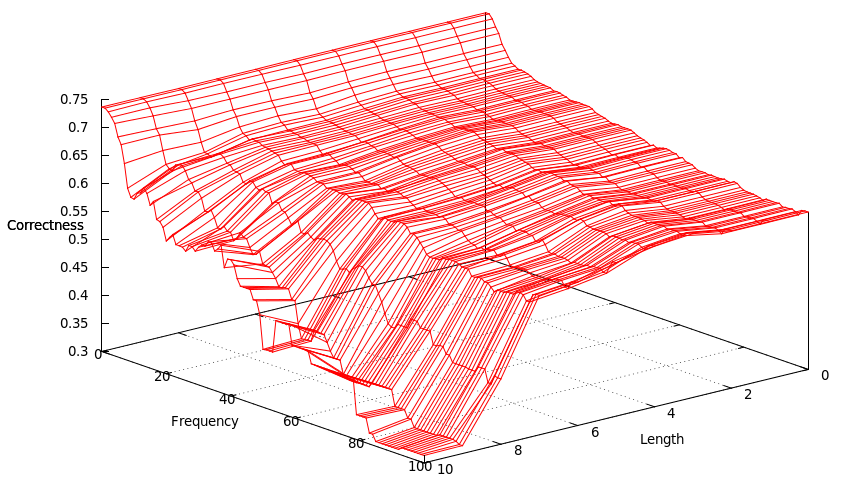
\includegraphics[width=140mm]{img/pak-paroubek-params.png}
\caption{Dobór parametrów algorytmu analizy sentymentu}
\label{image:pak-paroubek-parametry}
\end{figure}


\subsection{Wykrywanie zwolenników i przeciwników klubu}
\label{subsection:wykrywanie-zwolennikow}
Proces oznaczania użytkowników jako sympatyków i przeciwników drużyny przebiegał
w następujący sposób:
\begin{itemize}
  \item dla każdego użytkownika zliczono jego wpisy w meczach każdej z badanych 
  drużyn,
  \item jeśli w meczach drużyny A dla danego użytkownika przeważała liczba 
  wpisów pozytywnych, wówczas oznaczano takiego kibica jako zwolennika drużyny A,
  \item jeśli natomiast przeważała liczba wpisów negatywnych, wówczas taki kibic
  traktowany był jako przeciwnik danej drużyny.  
\end{itemize} 




\subsubsection{Ocena pozytywności wpisu}
W kilku miejscach została zastosowana miara pozytywności wpisu.
Została ona wyliczona przy pomocy następującego równania:

\begin{equation}
\label{equation:pozytywnosc}
P = \frac{|pos|}{|pos| + |neg|}
\end{equation}

gdzie:

$|pos|$ -- liczba wpisów oznaczonych jako pozytywne,

$|neg|$ -- liczba wpisów oznaczonych jako negatywne.


% %%%%%%%%%%%%%%%%%%%%%%%%%%%%%%%%%%%%%%%%%%%%%%%%%%% ANALIZA SIECI SPOŁECZNYCH
\section{Analiza sieci społecznych}
\label{section:siecispoleczne}
W tej sekcji przedstawiam zastosowane podejście do analizy sieci społecznych,
odkrywania sieci społecznych z zebranych danych oraz sposoby na wykrywanie grup
i badanie podobieństw między sieciami.
\subsection{Budowa sieci społecznych z danych z Twittera}
% wykorzystanie reply, retweet
Relacje między użytkownikami na Twitterze zbudowane są na modelu jednostronnym.
Oznacza to, że każdy posiada dwie listy -- osób, które obserwuje oraz osób,
przez które jest obserwowany (\textit{following} i \textit{followers}).
Są to listy statyczne, budowanie ręcznie przez użytkowników tego portalu
mikroblogowego. Twitter ukierunkowany jest jednak na swobodną komunikację między
wszystkimi użytkownikami -- dlatego kontakty między nimi nie są ograniczone
tylko do osób, które mamy na którejś z list. Nie ma żadnego problemu by jeden
użytkownik komunikował się z drugim, gdy oboje nie mają się na żadnej z list.
Najczęściej komunikacja ta odbywa się publicznie poprzez pisanie tweetów między
sobą, odpowiadanie na wpisy innych użytkowników. Aby uzyskać lepsze efekty
pokazując tworzące się grupy społeczne ukierunkowałem swoje prace na relacje
tworzone w trakcie interakcji między użytkownikami poprzez odpowiedzi i
retweety.

Streaming API dostarcza Tweet z następującymi polami: 
\begin{verbatim}
coordinates, favorited, truncated, created_at, id_str,
entities: {
  urls, hashtags, user_mentions
},
in_reply_to_user_id_str, contributors, text, retweet_count, 
in_reply_to_status_id_str, id, geo, retweeted, possibly_sensitive, 
in_reply_to_user_id, place,
user: {
  profile_sidebar_fill_color, profile_sidebar_border_color, 
  profile_background_tile, name, profile_image_url, created_at, 
  location, follow_request_sent, profile_link_color, is_translator,
  id_str, 
  entities: {
    url: {
      urls
    },
    description: {
      urls
    }
  },
  default_profile, contributors_enabled, favourites_count, url, 
  profile_image_url_https, utc_offset, id, 
  profile_use_background_image,  listed_count, profile_text_color, 
  lang, followers_count, protected, notifications, 
  profile_background_image_url_https, profile_background_color,
  verified, geo_enabled, time_zone, description,
  default_profile_image, profile_background_image_url, statuses_count,
  friends_count, following, show_all_inline_media, screen_name, 
},
in_reply_to_screen_name, source, in_reply_to_status_id
\end{verbatim} 

W polu \texttt{in\_reply\_to\_user\_id} znajdowuje się unikalny numer ID
użytkownika, do którego odpowiedź była skierowana, zaś w polu \texttt{user\_id}
ID autora odpowiedzi. 
Oprócz odpowiedzi istotne również były wpisy typu retweet. Przykładowy wpis tego
typu wygląda następująco: \texttt{RT @AHeryantooo: Keep calm and trust in Moyes. Gapapa Yes ;;)}.
Aby z takiego wpisu pobrać ID użytkownika, którego wpisu został retweetowany -- w tym
przypadku jest to użytkownik \texttt{@AHeryantooo}, przeglądałem tabelę z użytkownikami
i przypisywałem do tego rodzaju wpisów wartość pola \texttt{retweeted\_user\_id}
jako znalezione ID konkretnego użytkownika.

Korzystając z tych dwóch rodzajów połączeń między użytkownikami byłem w stanie 
odkryć relacje między nimi. Naturalnym rodzajem traktowania tych danych było
uznanie użytkowników (de facto ich numerów ID) za wierzchołki, a relacje między nimi
(\texttt{in\_reply\_to\_user\_id} oraz \texttt{retweeted\_user\_id}) za krawędzie
w grafie.

 \subsection{Wykrywanie grup i badanie podobieństwa}
 \label{section:koncepcja-wykrywaniegrup}
% gephi, modularity
Do wykrywania grup wśród sieci społecznych skorzystałem z narzędzia
otwartoźródłowego narzędzia \textit{Gephi} wspomagającego analizę grafową, w
którym został zaimplementowany algorytm przedstawiony w artykule
\cite{blondel2008fuc}. Przy jego użyciu konkretne węzły zostały podzielone
na grupy, nad którymi przeprowadzałem późniejsze analizy.


Grupy zostały zbudowane na podstawie relacji \textit{reply}
stworzonej z zebranych wpisów. Na podstawie odpowiedzi między różnymi
użytkownikami budowany był model sieci społecznej.
W każdym kolejnym meczu przeprowadzono badanie grup wśród użytkowników.
Uzyskane wyniki podzielono na trzy ,,koszyki''. W pierwszym znalazły się grupy 
3 lub 4 osobowe. W~drugim koszyku grupy mające od 5 do 9 osób, a w trzecim koszyku
większe grupy. 

Badanie podobieństwa oparte było o analizę kolejnych wydarzeń. 
Polegało na zliczeniu ile wierzchołków powtarza się w kolejnych meczach.
Oparte zostało o niniejsze równanie:
\begin{equation}
S = \frac{|V_1 \cap V_2|}{|V_1|}
\end{equation}  
gdzie:

$V_1$ -- zbiór wierzchołków w pierwszym wydarzeniu,

$V_2$ -- zbiór wierzchołków w drugim wydarzeniu.

Krótko mówiąc podobieństwo to iloraz liczby wspólnych wierzchołków między 
wydarzeniami a liczby wierzchołków w pierwszym z nich.

%%%%%%%%%%%%%%%%%%%%%%%%%%%%%%%%%%%%%%%%%%%%%%%%%%%%%%%%%%%%%%%%%%%%%%%%%%%%%%%%
%\begin{comment}
Badanie podobieństwa oparte było głównie o analizę kolejnych wydarzeń.
W tym celu zastosowałem dwa podejścia. Pierwsze oparte na wszystkich
wierzchołkach (użytkownikach) polegało na zliczeniu ile z nich się powtarza.
Podobieństwo między kolejnymi meczami zostało oparte o niniejsze równanie:
\begin{equation}
S = \frac{|V_1 \cap V_2|}{|V_1 \cup V_2|}
\end{equation}  
gdzie $V_i$ to zbiór wierzchołków w wydarzeniu $i$. Krótko mówiąc podobieństwo
to iloraz liczby wspólnych wierzchołków między wydarzeniami a liczby sumy 
wierzchołków tych wydarzeń.
Drugie podejście zostało zastosowane do znalezionych przy pomocy \textit{Gephi} 
grup. Bada ono podobieństwo pomiędzy grafami, uwzględniając zarówno wierzchołki
jak i krawędzie. Jest to opracowany przez mnie algorytm, który można wyrazić
wzorem:
\begin{equation}
S = \frac{E_1 \cap E_2}{E_{V_1 \cap V_2}} \cdot \frac{V_1 \cap V_2}{V_1 \cup V_2}
\end{equation}
gdzie $E_i$ oznacza krawędzie w grafie $i$, $V_i$ wierzchołki w grafie $i$,
natomiast $E_{V_1 \cap V_2}$ oznacza wszystkie krawędzie między wspólnymi 
wierzchołkami. Poniżej przedstawiam przykład zastosowania powyższego algorytmu.

\clearpage
Wyniki podobieństwa między grafami zaprezentowane są na rysunku 
\ref{image:podobienstwo-grafow}.

\begin{figure}[ht!]
\centering
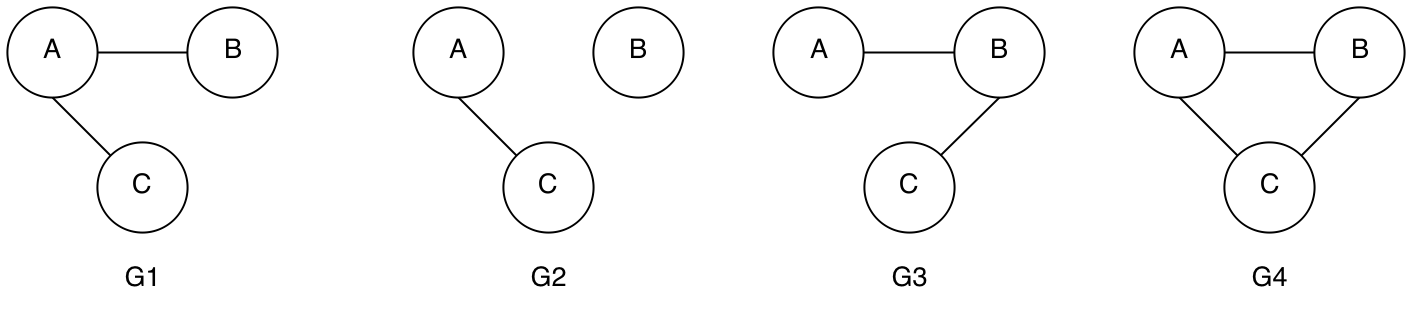
\includegraphics[width=140mm]{img/podobienstwo-grafow.png}
\caption{Przykładowe grafy do przedstawienia algorytmu podobieństwa}
\label{image:podobienstwo-grafow}
\end{figure}

\begin{table}[ht!]  
\begin{center}  
\begin{tabular}{|l|l|p{40mm}|p{40mm}||p{21mm}|}
\hline
Graf 1 & Graf 2 & Wsp. krawędzie / Krawędzie między wsp. wierzchołkami ($X_1$) & 
	Wsp. wierzchołki / Suma wierzchołków ($X_2$) & Podobieństwo ($X_1 \cdot X_2$)
\\ \hline 
G1 & G2 & 1 / 2 & 3 / 3 & 50.0 \% 
\\ \hline 
G1 & G3 & 1 / 3 & 3 / 3 & 33.3 \% 
\\ \hline 
G2 & G3 & 0 / 3 & 3 / 3 &  0.0 \%
\\ \hline 
G1 & G4 & 2 / 3 & 3 / 3 & 66.7 \%
\\ \hline
\end{tabular} 
\end{center} 
\caption{Przykładowe wyniki algorytmu podobieństwa grafów}
\end{table}

%\end{comment}

%%%%%%%%%%%%%%%%%%%%%%%%%%%%%%%%%%%%%%%%%%%%%%%%%%%%%% WYKORZYSTANIE GEOLOKACJI
\section{Wykorzystanie geolokacji}
\label{section:wykorzystaniegeolokacji}
% tweety z geolokacją
% wyciąganie informacji o miejscu - Open Street Map
% zastosowanie: odl. między użytkownikiami, od stadionu, dzielnice
W danych pobieranych z Twittera w części wpisów znajdowały się informacje o 
geolokacji -- współrzędne długości i szerokości geograficznej, z której
dany wpis został wysłany. Wykorzystanie tych informacji zostało zastosowane
do wzbogacenia analiz przeprowadzonych na zebranych danych. Informacje
o położeniu użytkowników bardzo często zbiegały się z miejscem rozgrywania meczu.
W bazie danych miałem jednak tylko informacje o danych geograficznych.
Aby wzbogacić je o więcej wiedzy postanowiłem skorzystać z projektu
Open Street Map (\textit{http://www.openstreetmap.org}).
Przy pomocy API, które projekt ten udostępnia udało mi się ubogacić dane
na temat lokalizacji o informacje opisowe miejsca, o które chodzi.
Poprzez \textit{Reverse Geocoding} możliwe było podając współrzędne
goegraficzne uzyskać między innymi takie informacji o adresie jak:
kraj (ang. \textit{country}), stan/państwo (ang. \textit{state}), 
hrabstwo (ang. \textit{county}), miasto (ang. \textit{city}).

Dodatkowo wykorzystanie geolokacji może być użyte do zbadania odległości między 
użytkownikami tworzącymi sieć społeczną, o tym w jakiej odległości są oni od stadionu,
czy również do zbadania sentymentu w zależności od wydarzeń na boisku,
a miejscem przebywania danych użytkowników. 



\subsection{Badanie odległości między użytkownikami}
\label{subsection:badanieodleglosci}
Badanie odległosci między użytkownikami odbyło się na podstawie odpowiedzi z
geolokacją -- retweety nie zawierają informacji o położeniu użytkownika.
Spośród tych użytkowników, którzy pisali z geolokacją zostało zliczone ilu z
nich się ze sobą komunikowało w zależności od wzajemnej odległości.








\end{comment}